\chapter{Full Datapath}


\section{Datapath}
In the WriteBack lab, you created a full non-pipelined datapath as shown in Fig~\ref{fig:datapath}.  The 5 integrated stages include:
\begin{enumerate}
\item iFetch
\item iDecode
\item iExecute
\item iMemory
\item iWriteBack
\end{enumerate} 

You verified your datapath by running your set of instructions in instrData.data and testing the output.  Each instruction should have executed as expected according to your Expected Results Table.

To further verify your datapath operation, you should create a new set of datafiles to implement the division code shown below.  You should first write assembly code, then translate it into binary.  One restriction is that the only non-zero value in your regData.data should be X22, which can be used as the base address for the array A.  Otherwise, all other data must be loaded from memory via the ramData.data and LDUR commands.  Please pay attention to the comments in division.c.

\Verilog{C code for doing simple division.}{code:division}{../code/division.c}

\begin{figure}
\caption{Full Non-Pipelined Datapath}\label{fig:datapath}
\begin{center}
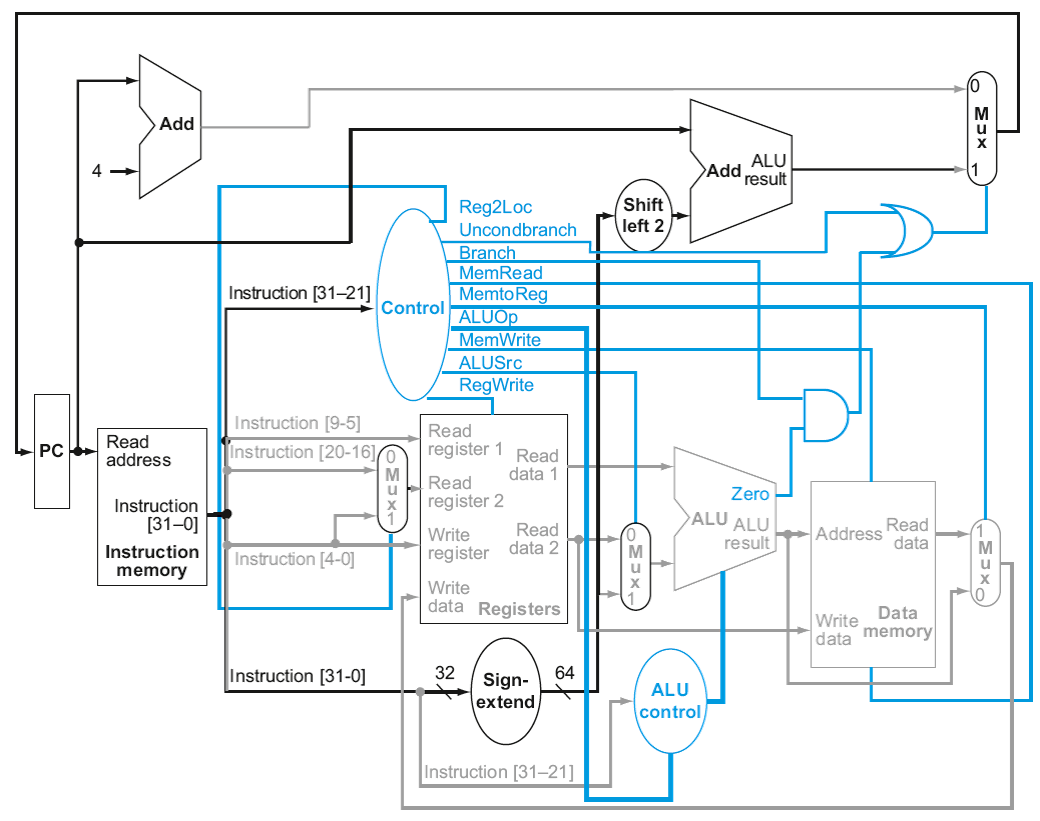
\includegraphics[width=\textwidth]{../images/non_pipelined_datapath.png}
\end{center}
\end{figure}

\section{Your Assignment}

You are to:
\begin{enumerate}
\item Implement the assembly and binary code for the Division C Code shown above.
\item Verify that the divison works correctly.
\item Write up a lab report according to a new format file, LabWriteup.tex.
\end{enumerate} 